\documentclass[a4paper]{report}
\usepackage{framed}%Used for the definition environment
\usepackage{enumerate}%Custom enumerates using \begin{enumerate}[yourListItem]
\usepackage{multicol}
\usepackage{amssymb}
\usepackage{amsmath}
\usepackage{mathtools}
\usepackage{todonotes}
\usepackage{cancel}
\usepackage[bookmarks,bookmarksdepth=2]{hyperref}%Depth of index in pdf program
\usepackage{tikz}
\usepackage{multicol}

%Environment for the definitions
\newenvironment{definition}[1]{\begin{framed}\centerline{\textbf{Definition #1}}\noindent\hspace{-1.1mm}}{\end{framed}}
\newtheorem{lemma}{Lemma}[chapter]

%Custom commands
\newcommand{\N}{\mathbb{N}}
\newcommand{\R}{\mathbb{R}}
\newcommand{\Z}{\mathbb{Z}}
\DeclarePairedDelimiter\cur{\{}{\}}
\renewcommand{\P}{\mathcal{P}}
\newcommand{\A}{\mathcal{A}}

\DeclarePairedDelimiter\abs{\lvert}{\rvert} % nice |x|
\DeclarePairedDelimiter\norm{\lVert}{\rVert} % nice ||x||
% Swap the definition of \abs* and \norm*, so that \abs
% and \norm resizes the size of the brackets, and the 
% starred version does not.
\makeatletter
\let\oldabs\abs
\def\abs{\@ifstar{\oldabs}{\oldabs*}}
\let\oldnorm\norm
\def\norm{\@ifstar{\oldnorm}{\oldnorm*}}
\makeatother




\begin{document}
\tableofcontents
\chapter{Introduction and Motivation}
\section{Discrete Mathematics and Computer Science}
Discrete Mathematics is concerned with finite and countably infinite mathematical structures. There are at least three major reasons why discrete mathematics is of central importance in computer science
\begin{itemize}
\item\textbf{Discrete structures}\\
Many objects studied in computer science are discrete mathematical objects, for example a graph modeling a computer network or an algebraic group used in cryptography. Many applications exploit sophisticated properties of the involved structures
\item\textbf{Abstraction}\\
A computer system can only be understood by considering a number of layers of abstraction, from application programs to the physical hardware
\item\textbf{Programs as mathematicals objects}\\
Understanding a computer program means to understand it as a discrete mathematical object
\end{itemize}
\section{Discrete Mathematics: A Selection of Teasers}
This section contains 8 examples, worth taking a look at.
\section{Abstraction: Simplicity and Generality}
In Discrete Mathematics, abstraction stands for simplicity and generality. In order to manage complexity, software systems are divided into components (called modules, layers, objects or abstract data types) that interact with each other and with the environment in a well-defined manner. \\

Abstraction means \emph{simplification}. By an abstraction one ignores all aspects of a system that are not relevant for the problem at hand, concentrating on the properties that matter\\

Abstraction also means \emph{generalization}. If one proves a property of a system described at an abstract level, then this property holds for any system with the same abstraction, independently of any details. 

\section{Programs as Discrete Mathematical Objects}
A computer program is a discrete mathematical object. The correctness of a program is a (discrete) mathematical statement. The proof that a program is correct (i.e., that it satisfies its specification) is a mathematical proof, not a heuristic argument. 

\chapter{Mathematical Reasoning, Proofs, and a First Approach to Logic} 
\section{What is a Proof?}
\setcounter{subsection}{1}
\subsection{The concept of a proof}
\begin{definition}{2.1 (Informal)} 
A \emph{proof} of a statement $S$ is a sequence of simple, easy verifiable consecutive steps. The proof starts from a set of axioms (things postulated to be true) and known (previously proved) facts. Each step corresponds to the application of a derivation rule to a few already proven statements, resulting in a newly proved statement, until the final step proves $S$.
\end{definition}
\subsection{Informal vs. Formal Proofs}
Formal Proof: Uses mathematical symbols and language.\\
Informal Proof: Explained using common, everyday language.\\

\noindent There are at least three (related) reasons for using a more rigurous and formal type of proof:
\begin{itemize}
\item \textbf{Prevention of errors}\\
A completely formal proof leaves no room for interpretation, and hence allows to exclude errors
\item \textbf{Proof complexity and automatic verification}\\
Certain proofs are too complex to be carried out and verified ``by hand''. A computer is required for the verification, which can only deal with rigurously formalized statements, not with semi-precise common language. 
\item\textbf{Precision and deeper understanding}\\
A formal proof requires the formalization of the arguments and can lead to a deeper understanding (also for the author of the proof).
\end{itemize}
\subsection{The Role of Logic}
Logic defines the syntax of language for expressing statements and the semantics of such a language, defining which statements are true and which are false. A logical calculus allows to express and verify proofs in a purely syntactic fashion, for example by a computer. 
\section{Propositions and Logical Formulas}
\subsection{Propositions, True and False}
\begin{definition}{2.2}
A proposition is a (mathematical) statement that is either \emph{true} or \emph{false}. Alternative terms for ``proposition'' are assertion, claim or simply statement. 
\end{definition}
Statements like ``Bob loves Carol'', ``it is raining'', and ``birds can fly'' are NOT (mathematical) propositions, unless we assume that the validity of these statements is defined (outside of mathematics, e.g. by common sense) to be a fixed, constant value (true or false).

\begin{definition}{2.3}
A true proposition is often called a \emph{theorem}, a \emph{lemma}, or a \emph{corollary}
\end{definition}
There is no fixed naming convention, but the term ``theorem'' is usually used for an important result, whereas a lemma is an intermediate, often technical result, possibly used in several subsequent proofs. A corollary is a simple consequence (e.g. a special case) of a theorem or lemma.

\subsection{Logical constants, Operators and Formulas}
\begin{definition}{2.4}
The Logical values (constants) ``true'' and ``false'' are usually denoted as 1 and 0, respectively. 
\end{definition}
\begin{definition}{2.5}
\begin{enumerate}[i)]
\item The \emph{negation} (Logical NOT) of a proposition $A$, denoted as $\lnot A$, is true if and only if $A$ is false.
\item The \emph{conjunction} (Logical AND) of two propositions $A$ and $B$, denoted $A\land B$, is true if and only if both $A$ and $B$ are true.
\item The \emph{disjunction} (Logical OR) of two propositions $A$ and $B$, denoted $A\lor B$, is true if and only if $A$ or $B$ (or both) are true
\end{enumerate}
\end{definition}
\begin{multicols}{3}
\null \vfill
\begin{displaymath}
\begin{array}{c||c}
   A
 & \lnot{}A \\
\hline
0 & 1 \\
1 & 0 \\
\end{array}
\end{displaymath}
\null \vfill
\columnbreak
\null \vfill
\begin{displaymath}
\begin{array}{c|c||c}
   A
 & B
 & A\land{}B \\
\hline
0 & 0 & 0 \\
0 & 1 & 0 \\
1 & 0 & 0 \\
1 & 1 & 1 \\
\end{array}
\end{displaymath}
\null \vfill
\columnbreak
\null \vfill
\begin{displaymath}
\begin{array}{c|c||c}
   A
 & B
 & A\lor{}B \\
\hline
0 & 0 & 0 \\
0 & 1 & 1 \\
1 & 0 & 1 \\
1 & 1 & 1 \\
\end{array}
\end{displaymath}
\null \vfill
\end{multicols}
Logical operators can also be combined, in the usual way of combining functions. For example, if A, B and C are propositions, then
\[ A\lor (B\land C)\] is also a proposition. Its function table is
\begin{displaymath}
\begin{array}{c|c|c||c}
   A
 & B
 & C
 & A\lor{}(B\land{}C) \\
\hline
0 & 0 & 0 & 0 \\
0 & 0 & 1 & 0 \\
0 & 1 & 0 & 0 \\
0 & 1 & 1 & 1 \\
1 & 0 & 0 & 1 \\
1 & 0 & 1 & 1 \\
1 & 1 & 0 & 1 \\
1 & 1 & 1 & 1 \\
\end{array}
\end{displaymath}
\begin{definition}{2.6}
A correctly formed expression involving propositional symbols (like $A,B,C,\dots$) and logical operators is called a \emph{formula} (of propositional logic)
\end{definition}
We introduce a new, derived logical operator: \emph{implication}, denoted as $A\to B$ and defined by\footnote{The symbol $:\Longleftrightarrow$ simply means that the left side (here $A\to B$) is defined to mean the right side (here $\lnot A\lor B$)}
\begin{multicols}{2}
\null\vfill
\[A\to B:\Longleftrightarrow\lnot A\lor B\]
\null\vfill
\columnbreak
\null\vfill
\begin{displaymath}
\begin{array}{c|c||c}
   A
 & B
 &A\to B \\
\hline
0 & 0 & 1 \\
0 & 1 & 1 \\
1 & 0 & 0 \\
1 & 1 & 1 \\
\end{array}
\end{displaymath}
\null\vfill
\end{multicols}
\subsubsection*{Example 2.2}
Consider the following sentence: If you read the lecture note every week and do the exercises ($A$), then you will get a good grade in the exam ($B$). This is an example of an implication $A\to B$. Saying that $A\to B$ is true does not mean that $A$ is true and it is not excluded that $B$ is true even if $A$ is false, but it is excluded that $B$ is false when $A$ is true.\\

\emph{Two-sided implication}, denoted $A\leftrightarrow B$, is defined as follows\footnote{Note that $A\equiv B$ holds if and only if $A\leftrightarrow B$ is true, but $A\equiv B$ itself is not a logical formula.}: 
\begin{multicols}{2}
\null\vfill
\[A\leftrightarrow B:\Longleftrightarrow (A\to B)\land (B\to A)\]
\null\vfill
\columnbreak
\null\vfill
\begin{displaymath}
\begin{array}{c|c||c}
   A
 & B
 & A\leftrightarrow B \\
\hline
0 & 0 & 1 \\
0 & 1 & 0 \\
1 & 0 & 0 \\
1 & 1 & 1 \\
\end{array}
\end{displaymath}
\null\vfill
\end{multicols}
Parenthesis can sometimes be dropped in a formula without changing its meaning, for example we can write $A\lor B\lor C$ instead of $A\lor (B\lor C)$ or $(A\lor B)\lor C$. Namely, $\land$ and $\lor$ bind stronger than $\to$ and $\leftrightarrow$. Also, $\lnot$ binds stronger than $\land$ and $\lor$. For example, we can write $A\lor \lnot B\to B\land C$ instead of $(A\lor (\lnot B))\to (B\land C)$
\subsection{Formulas as Functions and Logical Equivalence}
$(A\land (\lnot B))\lor (B\land(\lnot C))$ is a formula, and corresponds to a function $\{ 0,1\}^3\to\{ 0,1\}$.
\begin{definition}{2.7}
The symbol $\top$ denote a function that is the constant 1 (true), and $\perp$ denotes the function that is constant 0 (false).
\end{definition}
\begin{definition}{2.8}
Two Formulas $F$ and $G$ (in propositional logic) are called \emph{equivalent}, denoted as $F\Longleftrightarrow G$ (or also F$\equiv$ G), if they correspond to the same function (table).
\end{definition}
For example, it is easy to see that $\land$ and $\lor$ are commutative and associative, i.e. for any formulas $F,G,$ and $H$ we have 
\[F\land G\Longleftrightarrow G\land F \text{ and }  F\lor G\Longleftrightarrow G\lor F\]
as well as
\[ F\land (G\land H)\Longleftrightarrow (F\land G)\land H\Longleftrightarrow F\land G\land H\]
similarly 
\[ F\lor (G\lor H)\Longleftrightarrow (F\lor G)\lor H\Longleftrightarrow F\lor G\lor H\]
We also have 
\[\lnot( \lnot (F))\Longleftrightarrow F   \]

\subsection{Tautologies and Satisfiability}
\begin{definition}{2.9}
A formula $F$ (in propositional logic) is called a \emph{tautology} if it is true for all truth assignments of the involved propositional symbols. For example, the formulas $A\lor(\lnot A)$ and $(A\land (A\to B)\to B$ are tautologies
\end{definition}

\begin{definition}{2.10}
A formula $F$ (in propositional logic) is called \emph{satisfiable} if it is true for at least one truth assignment of the involved propositional symbols, and it is called \emph{unsatisfiable} otherwise
\end{definition}


\subsubsection*{Lemma 2.1}
{$F$ is a tautology if and only if $\lnot F$ is unsatisfiable.}
\subsection{The Symbols $\Longrightarrow$ and $\Longleftrightarrow$}
\begin{definition}{2.11}
One writes $F\Longrightarrow G$ (or $F\Rightarrow G$)(The length of the arrow is completely irrelevant) to say that $F$ implies $G$, i.e. that $F\to G$ is a tautology
\end{definition}
As mentioned earlier, one writes $F\Longleftrightarrow G$ if $F$ and $G$ imply each other, i.e. if $F$ and $G$ are equivalent. $F\Longleftrightarrow G$ is also expressed as ``$F$ if and only if $G$''.\\

To state $F\Longrightarrow G$ is the same as to state ``$F\to G$ is a tautology''. Note that $F\Longrightarrow G$ and $F\Longleftrightarrow G$ are not logical formulas since $\Longrightarrow$ and $\Longleftrightarrow$ are not allowed symbols in the syntax of logic. 
\subsubsection*{Theorem 2.2}
Implication is transitive: if $F\Longrightarrow G$ and $G\Longrightarrow H$, then $F\Longrightarrow H$\\

The theorem implies that, more generally, if one proves a statement $F_1$ as well as implications $F_1\Longrightarrow F_2, F_2\Longrightarrow F_3,\dots F_{n-1}\Longrightarrow F_n$, then one has proved $F_n$.

\section{Quantifiers and Predicate Logic}
The extension of propositional logic is called \emph{predicate logic} and is substantially more involved than propositional logic. 
\subsection{Predicates}
Let us consider a set $U$ as the universe in which we want to reason. For example, $U$ could be the set $\N$ of natural numbers, the set $\R$ of real numbers, the set $\{ 0,1\}*$ of finite-length bit-strings, or a finite set like $\{ 0,1,2,3,4,5,6\}$.

\begin{definition}{2.12}
A $k-$ary predicate $P$ on $U$ is a function $U^k\to\{ 0,1\}$
\end{definition}
A $k-$ary predicate $P$ assigns to each list $( x_1,\dots,x_k)$ of $k$ elements of $U$ the value $P(x_1,\dots, x_k)$ which is either true (1) or false (0).

\subsection{Definition of $\exists$ and $\forall$}
\begin{definition}{2.13}
For a universe $U$ and predicate $P(x)$ we define the following logical statements
\begin{itemize}
\item $\forall x P(x)$ is the statement that $P(x)$ is true for all $x\in U$
\item $\exists x P(x)$ is the statement that $P(x)$ is true for some $x\in U$, i.e. there exists an $x\in U$ for which $P(x)$ is true. 
\end{itemize}
\end{definition}
Sometimes one uses an abbreviated notation in which one specifies a condition for the variable $x$ directly. For example, we can write $\forall x\geq 5(x^2\geq 25)$ instead of $\forall x (x\geq 5)\to (x^2\geq 25)$.

\subsection{Nested Quantifiers}
Quantifiers can also be nested. For example, if $P(x)$ and $Q(x,y)$ are predicates, then \[\forall x(P(x)\lor\exists y  Q(y,x))\] is a logical formula.\\

\noindent\textbf{Check out multiple examples on page 19 about nested quantifiers}

\subsection{Tautologies and Satisfiability}
A formula is \emph{satisfiable} if, informally there is an interpretation that makes the formula true. Moreover, a formula is a \emph{tautology} if it is true for all interpretations, i.e. for all choices of the universe and for all interpretations of the predicates. For example:
\[\forall x ((P(x)\land Q(x))\to (P(x)\lor Q(x)))\]
is a tautology. As mentioned in section 2.2.5, we write $F\Longrightarrow G$ to mean that $F\to G$ is a tautology.\\

If the universe is fixed and there are no unspecified parts like predicate symbols, then a formula can trivially only be a tautology or unsatisfiable. 

\subsection{Some Rules}
We list a few useful rules for predicate logic
\begin{itemize}
\item $\forall x P(x)\land\forall x Q(x)\Longleftrightarrow \forall x(P(x)\land Q(x))$
\item $\exists x(P(x)\land Q(x))\Longrightarrow \exists x P(x)\land \exists x Q(x)$
\item $(\exists x P(x)\land \exists x Q(x))\to (\exists x(P(x)\land Q(x)))$ is not a tautology
\item $\lnot\forall xP(x)\Longleftrightarrow\exists x\lnot P(x)$
\item $\lnot\exists xP(x)\Longleftrightarrow\forall x\lnot P(x)$
\end{itemize}

\section{Some Proof Patterns and Techniques}
What is to be proven (e.g. a statement called a theorem) is given by a logical formula $F$, or by a sentence in natural language that could be made precise as (and hence stands for) a logical formula $F$. Typically $F$ is a proposition, i.e. it is either true or false, and for formulas in predicate logic the universe is understood. 
\subsection{Modus Ponens}
The following theorem states than in order to prove $G$ one can try to identify a formula $F$ such that one can prove both $F$ as well as $F\to G$. The proof is similar to the proof of theorem 2.2, using the fact that the propositional formula 
\[\left((A\land (A\to B)) \right)\to B\]
is a tautology. 
\subsubsection*{Theorem 2.3}
If $F$ and $F\to G$ are tautologies, then $G$ is also a tautology. 

\subsection{Direct Proof of an Implication}
\begin{definition}{2.14}
A \emph{direct proof} of an implication $F\to G$ works by assuming $F$ and then deriving $G$ (from $F$), where the derivation can possibly involve several proof steps. 
\end{definition}
\subsection{Indirect Proof of an Implication}
\begin{definition}{2.15}
An \emph{indirect proof} of an implication $F\to G$ works by assuming $\lnot G$ and deriving $\lnot F$, i.e. by proving $\lnot G\to \lnot F$
\end{definition}
This is correct because $F\to G$ id logically equivalent to $\lnot G\to\lnot F$, i.e. \[F\to G\Longleftrightarrow \lnot G\to\lnot F\]

\subsection{Proofs by Contradiction}
The following theorem states that in order to prove $F$ one can try to identify a formula $G$ such that one can prove both $\lnot G$ as well as $\lnot F\to G$. The proof is similar to the proof of Theorem 2.2, using the fact that the propositional formula 
\[\left( (\lnot A\to B)\land \lnot B\right)\to A\]
is a tautology.
\subsubsection*{Theorem 2.4}
If $\lnot F\to G$ and $\lnot G$ are tautologies, then $F$ is also a tautology (or: If $\lnot F \to\perp$ is a tautology, then $F$ is also a tautology. \\

Such proof usually works by assuming $\lnot F$, and deriving from this assumption a formula $H$ and also its negation $\lnot H$, which is a contradiction. In other words, one proves $\lnot F\to H$ as well as $\lnot F\to \lnot H$, and hence also $\lnot F\to (H\land\lnot H)$, i.e. the formula $G$ of the theorem is $G=H\land \lnot H$

\subsection{Existence Proofs}
\begin{definition}{2.16}
An existence proof is the proof of a statement of the form $\exists x P(x)$
\end{definition}
There are constructive existence proofs, which demonstrate an $a$ for which $P(a)$ is true, as well as non-constructive existence proofs which simply show the existence of an $a$ for which $P(a)$ is true, without exhibiting such an $a$.

\subsection{Inexistence Proofs}
\begin{definition}{2.17}
An inexistence proof is a proof of a statement of the form $\lnot \exists x P(x)$
\end{definition}
To prove the inexistence, one can use \[\lnot\exists x P(x)\Longleftrightarrow \forall x\lnot P(x)\]

\subsection{Proofs by Counterexample}
\begin{definition}{2.18}
A proof by counterexample is a proof of a statement of the form $\lnot\forall x P(x)$ for some fixed predicate $P$, using \[\lnot \forall x P(x)\Longleftrightarrow \exists x\lnot P(x)\]
An $a$ for which $\lnot P(a)$ is true is called a counterexample
\end{definition}

\subsection{Proofs by Induction}
A proof by induction consists in two steps:
\begin{enumerate}
\item \textbf{Basis Step}: Prove $P(0)$
\item \textbf{Induction Step}: Prove $\forall n(P(n)\to P(n+1))$
\end{enumerate}
\subsubsection*{Theorem 2.5}
For every predicate $P$ on $\N$ we have \[P(0)\land\forall n(P(n)\to P(n+1))\Longrightarrow \forall n P(n)\]

\subsubsection*{Fact 2.1}
The natural numbers are well-ordered, i.e. every nonempty set of natural numbers has a least element\footnote{The well-ordering principle could be stated more formally as \[\exists n P(n)\Longrightarrow \exists m \left( P(m)\land \forall k <m\lnot P(k)\right)\] but we will not need this formula.}

\chapter{Sets, Relations and Functions}
There seems to be no simpler mathematical concept than a \emph{set} (Menge), a collection of objects.\\

\emph{``Unter eine Menge verstehen wir jede Zusammenfassung $M$ von bestimmten wohlunterschiedenen Objekten unserer Anschauung oder unseres Denkens (welche die Elemente von $M$ genannt werden) zu einem Ganzen''} - Georg Cantor, 1895

\section{Sets and Operations on Sets}
\subsection{Set Memebership, Set Equality, and Cardinality}
We assume that for every object $x$ and set $A$ it is defined whether $x$ is an \emph{element} of $A$, denoted $x\in A$, or whether it is not an element of $A$, denoted $x\not\in A$ (instead of $\lnot(x\in A))$

\subsubsection*{Example 3.1}
If $\Z$ denotes the set of integers, then $5\in \Z$, but $\frac{1}{2}\not\in\Z$. Two sets $A$ and $B$ are equal $(A=B)$ if and only if they contain the same elements, independently of how $A$ and $B$ are described.

\begin{definition}{3.1}
\[A=B:\Longleftrightarrow\forall x(x\in A\leftrightarrow x\in B)\]
\end{definition}
\begin{definition}{3.2}
The number of elements of a finite set $A$ is called its \textbf{cardinality} and is denoted $\abs{A}$
\end{definition}

\subsection{Set Description}
A natural way to specify a finite set is by listing its elements. We use the standard notation $A=\{a,b,c\}$ to say that the set contains the three elements $a,b,c$ and no other element. If two elements in the list are equal, then one of them an be dropped. 

\subsubsection*{Example 3.2}
\[\{1,2,3\}=\{1,2,3,1,3\}=\{3,1,2\}=\left\{2,\frac{18}{6},\frac{6}{3},1\right\}\]
A set can also be described by defining a property of its elements. If $A$ is a set and $P$ is a predicate defined on $A$, then \[\{x\in A\mid P(x)\}\] which denotes the set of elements of $A$ having property $P$

\subsubsection*{Example 3.3}
For $A=\{n\in\Z\mid 1\leq n\leq 10\}$ we have $\{n\in A\mid\text{ prime($n$)}\}=\{2,3,5,7\}$

\subsection{Sets as Elements}
Sets can themselves be elements of a set. For example, the set $\cur{3,\cur{4,5}}$ is a set with two elements, the number 3 and the set $\cur{4,5}$.\\

For the operation of forming an \emph{ordered pair} of two objects $a$ and $b$, denoted $(a,b)$, we have \[(a,b)=(c,d):\Longleftrightarrow a=c\land b=d\]

\subsection{Subsets}
An important relation between sets is the \emph{subset} (or \emph{inclusion}) relation.

\begin{definition}{3.3}
The set $A$ is a subset of the set $B$, denoted $A\subseteq B$, if every element of $A$ is also an element of $B$, i.e. \[A\subseteq B:\Longleftrightarrow\forall x(x\in A\to x\in B)\]
\end{definition}

\subsection{The Empty Set}
\begin{definition}{3.4}
The \emph{empty set}, denoted $\varnothing$ or $\cur{}$, is the set with no elements, i.e. $\forall x (x\not\in\varnothing)$
\end{definition}

\subsubsection*{Lemma 3.1}
The empty set is a subset of every set, i.e. $\forall A (\varnothing\subseteq A)$.

\subsubsection*{Lemma 3.2}
The empty set is unique.

\subsection{Constructing Sets form the Empty Set}
The empty set can be used to construct new sets, without using any other predefined objects as elements. The set $\cur{\varnothing}$ is a set with a single element, the empty set $\varnothing$. It is important not to confuse $\varnothing$ with $\cur{\varnothing}$. Note that $\abs{\cur{\varnothing}}=1$ while $\abs{\varnothing}$. Sets with different (finite) cardinality are different. One can define a whole sequence of such sets:
\[\varnothing,\cur{\varnothing},\cur{\cur{\varnothing}}\cur{\cur{\cur{\varnothing}}},\dots\] 
Note that except for the empty set, all these sets have cardinality 1.

\subsection{The Power Set}
\begin{definition}{3.5}
The \emph{power set} of a set $A$, denoted $\P(A)$ or sometimes $2^A$, is the set of all subsets of $A$: \[\P(A):=\cur{S\mid S\subseteq A}\]
\end{definition}
For a finite set with cardinality $k$, the power set has cardinality $2^k$ (hence the name 'power set' and the alternative notation $2^A$)

\subsection{Union, Intersection, Difference and Complement}
\begin{definition}{3.6}
The \emph{union} of two sets $A$ and $B$ is defined as 
\[A\cup B:=\cur{x\mid x\in A\lor x\in B}\text{ or }\forall x(x\in A\cup B\leftrightarrow x\in A\lor x\in B)\]
and their \emph{intersection} is defined as 
\[A\cap B:=\cur{x\mid x\in A\land x\in B}\]
\end{definition}

Let $\A$ be a set of sets, with finite or infinite cardinality. The only restriction on $\A$ is that its elements must be sets. Then we define the union of all sets in $\A$ as the set of all $x$ that are an element of at least one of the sets in $\A$:
\[\bigcup {\A} :=\cur{x\mid\exists A\in A:x\in A}\]
Similarly, we define the intersection of all sets in $\A$ as the set of all $x$ that are an element of every set in $\A$:
\[\bigcap {\A} :=\cur{x\mid\forall A\in A:x\in A}\]

\begin{definition}{3.7}
For a given universe of discourse $U$, the \emph{complement} of a set $A$, denoted $\overline{A}$ is \[\overline{A}:=\cur{x\in U\mid x\not\in A}\] or simply $\overline{A}=\cur{x\mid x\not\in A}$\footnote{The complement of $A$ is sometimes also denoted as $A^c$}.\\

If union and intersection are understood as logical OR and AND, respectively, then the complement can be understood as the logical negation.
\end{definition}
\todo[inline]{Problem with footnote inside framed environment!!}

\begin{definition}{3.8}
The \emph{difference} of sets $B$ and $A$, denoted $B-A$ (or sometimes $B\backslash A$) is the complement of $A$, relative to $B$: \[B-A:=\cur{x\in B\mid x\not\in A}\] 
\end{definition}

\subsubsection*{Theorem 3.3}
For any sets $A,B$ and $C$, and a universe $U$, the following laws hold:\\
\begin{center}
\begin{tabular}{r l}
Idempotence: & $A\cap A=A$ \\
{}& $A\cup A=A$\\
Commutativity: & $A\cap B=B\cap A$\\
{}&$A\cup B=B\cup A$\\
Associativity: & $A\cap (B\cap C)=(A\cap B)\cap C$\\
{} & $A\cup (B\cup C)=(A\cup B)\cup C$\\
Absorption: & $A\cap (A\cup B)=A$\\
{}& $A\cup (A\cap B)=A$\\
Distributivity: & $A\cap (B\cup C)=(A\cap B)\cup (A\cap C)$\\
{}&$A\cup (B\cap C)=(A\cup B)\cap (A\cup C)$\\
Complementarity: & $A\cap\overline{A}=\varnothing$\\
{} & $A\cup\overline{A}= U$\\
Consistency: & $A\subseteq B\Longleftrightarrow A\cap B=A\Longleftrightarrow A\cup B=B$
\end{tabular}
\end{center}

\subsection{The Cartesian Product}
\begin{definition}{3.9}
The \emph{Cartesian product} $A\times B$ of two sets $A$ and $B$ is the set of all ordered pairs with the first component from $A$ and the second component from $B$: \[A\times B=\cur{(a,b)\mid a\in A\land b\in B}\]
\end{definition}
For finite sets, the cardinality of the Cartesian product of some sets is the product of their cardinalities.

\subsection{Russell's Paradox}
The problem with Cantor's intuitive set theory is that, because it was not clearly axiomatized, it makes the following apparently innocent (yet false) assumption. Whenever one specifies a precise condition, allowing to distinguish between objects that satisfy the condition and objects that don't, then $\cur{x\mid P(x)}$, the set of objects satisfying the definition, is well-defined. Russell proposed the set \[R=\cur{A\mid A\not\in A}\] of sets that are not themselves. Note that there seems nothing wrong with a set being an element of itself. For example, the set of sets containing at least 10 elements is certainly an element of itself, as it contains 10 elements. 
\todo[inline]{Check again, maybe find a better and shorter explanation}
\section{Relations}
\subsection{The Relation Concept}
\begin{definition}{3.10}
A (binary) relation $\rho$ from a set $A$ to a set $B$ is a subset of $A\times B$. If $A=B$, then $\rho$ is called a relation on $A$
\end{definition}
Instead of $(a,b)\in \rho$ one usually writes \[a\rho b\] and sometimes we write $a\cancel{\rho} b$ if $(a,b)\not\in\rho$

\subsection{Representations of Relations}
For finite sets $A$ and $B$, a (binary) relation $\rho$ from $A$ to $B$ can be represented as a Boolean $\abs{A}\times\abs{B}$ matrix $M^\rho$ with the rows and columns labeled by the elements of $A$ and $B$ respectively. For $a\in A$ and $b\in B$, the matrix entry $M_{a,b}^\rho$ is 1 if $a\rho b$, 0 otherwise.

\subsection{Set Operations on Relations}
Relations are sets, and therefore we can apply any operation defined on sets: union, intersection and complement. 

\subsection{The Inverse of a Relation}
\begin{definition}{3.12}
The \emph{inverse} of a relation $\rho$ from $A$ to $B$ is the relation $\widehat{\rho}$ from $B$ to $A$ such that \[a\rho b\Longleftrightarrow b\widehat{\rho} a\]
\end{definition}
An alternative notation for the inverse of $\rho$ is $\rho^{-1}$\\

In the matrix representation, taking the inverse of a relation corresponds to the transposition of the matrix. In the graph representation, it taking the inverse corresponds to inverting the direction of all edges.

\subsection{Composition of Relations}
\begin{definition}{3.13}
Let $\rho$ be a relation from $A$ to $B$ and let $\sigma$ be a relation from $B$ to $C$. Then the \emph{composition} of $\rho$ and $\sigma$, denoted $\rho\sigma$ (or also $\rho\circ\sigma$), is the relation from $A$ to $C$ where \[a\rho\sigma c:\Longleftrightarrow\exists b\in B:(a\rho b\land b\sigma c)\]
The $n-$fold composition of a relation $\rho$ on a set $A$ is denoted $\rho^n$
\end{definition}

\subsubsection*{Lemma 3.4}
The composition of relations is associative, i.e. we have $\rho(\sigma\phi)=(\rho\sigma)\phi$

\subsubsection*{Lemma 3.5}
Let $\rho$ be a relation from $A$ to $B$ and let $\sigma$ be a relation from $B$ to $C$. Then the inverse $\widehat{\rho\sigma}$ of $\rho\sigma$ is the relation $\widehat{\sigma}\widehat{\rho}$

\subsection{Special Properties of Relations}
\begin{definition}{3.14}
A relation $\rho$ on a st $A$ is called \emph{reflexive} if $a\rho a$ for every $a\in A$, i.e. if $\text{id}\subseteq\rho$
\end{definition}
In other words, a relation is reflexive if it contains the equality relation ($=$). In the matrix representation of relations, reflexive means that the diagonal is all 1. In a graph representation, reflexive means that every vertex has a loop (an edge from the vertex to itself).

\begin{definition}{3.16}
A relation $\rho$ on a set $A$ is called \emph{symmetric} if $\rho=\widehat{\rho}$, i.e. if \[a\rho b\Longleftrightarrow b\rho a\]
\end{definition}
In the matrix representation of relations, symmetric means that the matrix is symmetric (with respect to the diagonal).

\begin{definition}{3.17}
A relation $\rho$ on a set $A$ is called \emph{antisymmetric} if $\rho\cap\widehat{\rho}\subseteq\text{id}$, i.e. \[a\rho b\land b\rho a\Longrightarrow a=b\]
\end{definition}
In a graph representation, antisymmetric means that there is no cycle of length 2, i.e. no distinct vertices $a$ and $b$ with edges both from $a$ and $b$ and from $b$ to $a$. Note that antisymmetric is \textbf{not} the negation of symmetric. 

\begin{definition}{3.18}
A relation $\rho$ on a set $A$ is called \emph{transitive} if \[a\rho b\land b\rho c\Longrightarrow a\rho c\]
\end{definition}

\subsubsection*{Lemma 3.6}
A relation $\rho$ is transitive if and only if $\rho^2\subseteq\rho$.

\subsection{Transitive Closure}
\begin{definition}{3.19}
The transitive closure of a relation $\rho$ on a set $A$, denoted $\rho^*$, is \[{\rho ^*} = \bigcup\limits_{n = 1}^\infty  {{\rho ^n}} \]
\end{definition}
In the graph representation of a relation $\rho$ on $A$, we have $a\rho^k b$ if and only if there is a path of length $k$ from $a$ to $b$ in the graph. The transitive closure is the reachability relation, i.e. $a\rho^* b$ if and only if there is a path (of arbitrary finite length) from $a$ to $b$.

\section{Equivalence Relations}
\subsection{Definition of Equivalence Relations}
\begin{definition}{3.20}
An \emph{equivalence relation} is a relation that is reflexive, symmetric and transitive 
\end{definition}

\begin{definition}{3.21}
For an equivalence relation $\theta$ on a set $A$ and for $a\in A$, the set of elements of $A$ that are equivalent to $a$ is called the \emph{equivalence class of} a and is denoted as $\lbrack a\rbrack_\theta$: \[\lbrack a\rbrack_\theta:=\cur{b\in A\mid b\theta a}\]
\end{definition}

\subsubsection*{Lemma 3.7}
The intersection of two equivalence relations is an equivalence relation.

\subsubsection*{Example 3.44}
The intersection of $\equiv_5$ and $\equiv_3$ is $\equiv_{15}$.

\subsection{Equivalence Classes Form a Partition}
\begin{definition}{3.22}
A \emph{partition} of a set $A$ is a set $\cur{S_i\subseteq A}_{i\in I}$ of mutually disjoint subsets of $A$ that cover $A$, i.e. \[S_i\cap S_j=\varnothing\hspace{5mm}\text{for }i\not= j\hspace{7.5mm}\text{and}\hspace{7.5mm}\bigcup\limits_{i\in I}S_i=A\]
\end{definition}
Partitions and equivalence relations capture the same (simple) abstraction.

\begin{definition}{3.23}
The set of equivalence classes of an equivalence relation $\theta$, denoted by \[A/\theta:=\cur{\lbrack a\rbrack_\theta\mid a\in A}\] is called the \emph{quotient set of} $A$ by $\theta$, or simply $A$ modulo $\theta$, or $A$ mod $\theta$.
\end{definition}

\subsubsection*{Theorem 3.8}
The set $A/\theta$ of equivalence classes of an equivalence relation $\theta$ on $A$ is a partition of $A$.

\todo[inline]{Maybe add proof on page 45}
\subsection{Example: Definition of the Rational Numbers}
\todo[inline]{send back to the book!}

\section{Partial Order Relations}
\subsection{Definition}
\begin{definition}{3.24}
A \emph{partial order} on a set $A$ is a relation that is reflexive, antisymmetric and transitive. A set $A$ together with a partial order $\preceq$ on $A$ is called a \emph{partially ordered set} (or simply \emph{poset}) and is denoted as $(A;\preceq)$\footnote{Partial orders are usually denoted by $\leq$ or by a similar symbol}
\end{definition}

In a graph representation of relations, a partial order has no cycles. \\

For a partial order relation $\preceq$ we can define the relation $a\prec b$ similar to how the relation $<$ is obtained from $\leq$: \[a\prec b:\Longleftrightarrow a\preceq b\land a\not=b\]

\begin{definition}{3.25}
For a poset $(A;\preceq)$, two elements $a$ and $b$ are called \emph{comparable} if $a\preceq b$ or $b\preceq a$; otherwise they are called \emph{incomparable}
\end{definition}

\begin{definition}{3.26}
If any two elements of a poset $(A;\preceq)$ are comparable, then $A$ is called \emph{totally ordered} (or \emph{linearly ordered} by $\preceq$
\end{definition}

\begin{definition}{3.27}
A poset $(A;\preceq)$ is \emph{well-ordered} if it is totally ordered and if every non-empty subset of $A$ has a least element
\end{definition}

Note that every totally ordered finite poset is well-ordered. The property of being well-ordered is of interest inly for infinite posets. Any subset of the natural numbers is also well-ordered. 

\subsection{Hasse Diagrams}
\begin{definition}{3.28}
In a poset $(A;\preceq)$ an element $b$ is said to \emph{cover} an element $a$ if $a\prec b$ and there exists no $c$ with $a\prec c$ and $c\prec b$ (i.e. between $a$ and $b$)
\end{definition}

\begin{definition}{3.29}
The \emph{Hasse diagrams} of a (finite) poset $(A;\preceq)$ is the directed graph whose vertices are labeled with the elements of $A$ and where there is an edge from $a$ to $b$ if and only if $b$ covers $a$
\end{definition}

The Hasse diagram is a graph with directed edges. It usually drawn such that whenever $a\prec b$, then $b$ is placed higher than $a$. This means that all arrows are directed upwards ad therefore can be omitted.

\begin{center}
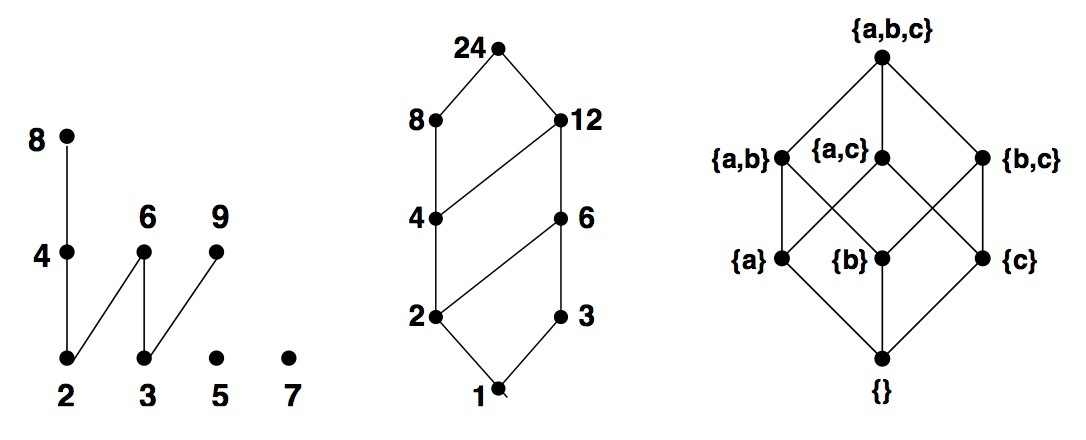
\includegraphics[scale=0.27]{Figures/Figure3,1Page48.jpg}
\end{center}

\subsection{Chains and Antichains}
\begin{definition}{3.30}
A totally ordered subset (with respect to $\preceq$) $C\subseteq A$ of a poset $(A;\preceq)$ is called a chain (in$(A;\preceq)$)
\end{definition}

\begin{definition}{3.31}
A subset $B\subseteq A$ of a poset $(A;\preceq)$ is called an \emph{antichain} if any two distinct elements in $B$ are incomparable
\end{definition}

\subsection{Combinations of Posets and the Lexicographic Order}
\subsubsection*{Theorem 3.9}
For given posets $(A;\preceq)$ and $(B;\sqsubseteq)$, the relation $\leq_\text{lex}$ defined on $A\times B$ by \[(a_1,b_1)\leq (a_2,b_2):\Longleftrightarrow a_1\preceq a_2\land b_1\sqsubseteq b_2\]
is a partial order relation.

\subsubsection*{Theorem 3.10}
For given posets $(A;\preceq)$ and $(B;\sqsubseteq)$, the relation $\leq_\text{lex}$ defined on $A\times B$ by \[(a_1,b_1)\leq_\text{lex} (a_2,b_2):\Longleftrightarrow a_1\prec a_2\lor (a_1=a_2\land b_1\sqsubseteq b_2)\]
is a partial order relation.\footnote{As mentioned earlier, for a partial order $\preceq$ we can define the relation $\prec$ as $a\prec b:\Longleftrightarrow a\preceq b\land a\not=b$}

\subsection{Special elements in Posets}
\begin{definition}{3.32}
Let $(A;\preceq)$ be a poset, and let $S\subseteq A$ be some subset of $A$. Then 
\begin{enumerate}
\item $a\in S$ is a \emph{minimal (maximal) element} of $S$ if there exists no $b\in S$ with $b\prec a$ $(b\succ a)$
\item $a\in S$ is the \emph{least (greates) element} of $S$ if $a\preceq b$ $(a\succeq b)$ for all $b\in S$
\item $a\in A$ is a \emph{lower (upper) bound} of $S$ if $a\preceq b$ $(a\succ b)$ for all $b\in S$
\item $a\in A$ is the \emph{greatest lower bound (least upper bound)} of $S$ if $a$ is the greatest (least) element of the set of all lower (upper) bounds of $S$ 
\end{enumerate}
\end{definition}
Minimal, maximal, least and greatest elements are easily identified in a Hasse diagram. \\
\indent The greatest lower bound and the least upper bound of a set $S$ are sometimes denotes as glb$(S)$ and lub$(S)$, respectively. 
\subsection{Meet, Join and Lattices}
\begin{definition}{3.33}
Let $(A;\preceq)$ be a poset. If $a$ and $b$ (i.e. the set $\{a,b\}\subseteq A$) have a greatest lower bound, then it is called the \emph{meet} of $a$ and $b$, often denoted $a\land b$. If $a$ and $b$ have a least upper bound, then it is called the \emph{join} of $a$ and $b$, often denoted $a\lor b$.
\end{definition}

\begin{definition}{3.34}
A poset $(A;\preceq)$ in which every pair of elements has a meet and a join is called a \emph{lattice}
\end{definition}

\section{Functions}
\subsection{The Function Concept}
\begin{definition}{3.35}
A function $f:A\to B$ from a \emph{domain} $A$ to a \emph{codomain} $B$ is a relation $A\times B$, i.e. a subset $f\subseteq A\times B$, with the special properties (using the relation notation $afb$):
\begin{enumerate}
\item $\forall a\in A \hspace{2mm} \exists b\in B\hspace{2mm} afb$\hspace{10mm}($f$ is totally defined)
\item $afb\land afb'\hspace{2mm}\Rightarrow b=b'$\hspace{9mm}($f$ is well-defined)
\end{enumerate}
\end{definition}
The set of all functions $A\to B$ is denoted as $B^A$. This notation is motivated by the fact that if $A$ and $B$ are finite, then there are $\abs{B}^{\abs{A}}$ such functions (see Section 4.1).

\begin{definition}{3.36}
A \emph{partial function} is a relation $A\times B$ such that condition 2. above holds
\end{definition}

\begin{definition}{3.37}
Two (partial) functions with common domain $A$ and codomain $b$ are \emph{equal} if they are equal as relations (i.e. as sets)
\end{definition}

$f=g$ is equivalent to saying that the function values of $f$ and $g$ agree for all arguments (including, in case of partial functions, whether or not it is defined)

\begin{definition}{3.38}
For a function $f:A\to B$ and a subset $S$ of $A$, the \emph{image} of $S$ under $f$, denoted $f(S)$, is the set \[f(S):=\{f(a)\mid a\in S\}\]
\end{definition}

\begin{definition}{3.39}
The subset $f(A)$ of $B$ is called the \emph{image} (or \emph{range}) of $f$ and is also denoted $\text{Im}(f)$
\end{definition}

\begin{definition}{3.40}
For a subset $T$ of $B$, the \emph{inverse image} (or \emph{preimage}) of $T$, denoted $f^{-1}(T)$, is the set of values in $A$ that map into $T$: \[f^{-1}(T):=\{a\in A\mid f(a)\in T\}\]
\end{definition}


\subsection{Properties of Functions and Function Composition}
\begin{definition}{3.41}
A function $f:A\to B$ is called
\begin{enumerate}
\item \emph{Injective} if $a\not=b\Rightarrow f(a)\not=f(b)$, i.e. no two distinct values are mapped to the same function value (there are no ``collisions'')
\item \emph{Surjective} (or \emph{onto}) if for every $b\in B$, $b=f(a)$ for some $a\in A$, i.e. if $f(A)=B$ (every value in the codomain is taken on for some argument)
\item \emph{Bijective} if it is both surjective and injective.  
\end{enumerate}
\end{definition}

\begin{definition}{3.42}
The \emph{composition} of a function $f:A\to B$ and a function $g:B\to C$, denoted by $g\circ f$, or simply $gf$, is defined by $g\circ f(a)=g\left( f(a)\right)$
\end{definition}

\subsubsection*{Lemma 3.11}
Function composition is associative, i.e. $(h\circ g)\circ f = h\circ (g\circ f)$

\chapter{Combinatorics and Counting}













\end{document}